
\documentclass[aspectratio=169, handout]{beamer}

%\usepackage[table]{xcolor}
\mode<presentation> {
\setbeamercovered{transparent}
  \usetheme{Boadilla}

\usepackage{booktabs}
\renewcommand{\familydefault}{cmss}

\useinnertheme{rectangles}
}

\usepackage{bm}
\usepackage{amsmath}
\usepackage{bbold}
\setbeamercolor{normal text}{fg=black}
\setbeamercolor{structure}{fg= blue}
\definecolor{trial}{cmyk}{1,0,0, 0}
\definecolor{trial2}{cmyk}{0.00,0,1, 0}
\definecolor{darkgreen}{rgb}{0,.4, 0.1}
\usepackage{array}
\definecolor{darkpurple}{rgb}{0.4, 0, 0.6}
\beamertemplatesolidbackgroundcolor{white}  \setbeamercolor{alerted
text}{fg=darkpurple}
\usepackage{tcolorbox}
\setbeamertemplate{caption}[numbered]\newcounter{mylastframe}

\usepackage{tikz}
\usetikzlibrary{arrows}
\usepackage{colortbl}
\usepackage{pgfplots}
\pgfplotsset{compat=1.17}

\renewcommand{\familydefault}{cmss}

\usepackage{lipsum}

 \newenvironment{changemargin}[3]{%
 \begin{list}{}{%
 \setlength{\topsep}{0pt}%
 \setlength{\leftmargin}{#1}%
 \setlength{\rightmargin}{#2}%
 \setlength{\topmargin}{#3}%
 \setlength{\listparindent}{\parindent}%
 \setlength{\itemindent}{\parindent}%
 \setlength{\parsep}{\parskip}%
 }%
\item[]}{\end{list}}
\usetikzlibrary{arrows}

\usecolortheme{lily}
% Math operators
\DeclareMathOperator{\tr}{tr}
\DeclareMathOperator{\rank}{rank}
\DeclareMathOperator{\col}{col}
\DeclareMathOperator{\spn}{span}
\newtheorem{com}{Comment}
\newtheorem{lem} {Lemma}
\newtheorem{prop}{Proposition}
\newtheorem{condition}{Condition}
\newtheorem{thm}{Theorem}
\newtheorem{defn}{Definition}
\newtheorem{cor}{Corollary}
\newtheorem{obs}{Observation}
 \numberwithin{equation}{section}

\makeatletter
\def\beamerorig@set@color{%
  \pdfliteral{\current@color}%
  \aftergroup\reset@color
}
\def\beamerorig@reset@color{\pdfliteral{\current@color}}
\makeatother
\setbeamertemplate{navigation symbols}{}

\useoutertheme{miniframes}
\makeatletter
\setbeamertemplate{headline}
{%
  \begin{beamercolorbox}[colsep=1.5pt]{upper separation line head}
  \end{beamercolorbox}
  \begin{beamercolorbox}{section in head/foot}
    \vskip2pt\insertnavigation{\paperwidth}\vskip2pt
  \end{beamercolorbox}%
  \ifbeamer@theme@subsection%
    % Removed subsection navigation
  \fi%
  \begin{beamercolorbox}[colsep=1.5pt]{lower separation line head}
  \end{beamercolorbox}
}
\makeatother

\title[PLSC 30700]{Linear Models: Probability and Linear Algebra Review}

\author{Robert Gulotty}
\institute[Chicago]{University of Chicago}
\vspace{0.3in}



\begin{document}


\begin{frame}
\maketitle
\end{frame}

\begin{frame}{Two Ways an Empirical Project Can Fail}

\vspace{0.2cm}

\textbf{1) Identification Failure}

\begin{itemize}
    \item The causal parameter (e.g. $\tau$) is not uniquely determined by the observable data.
    \item Multiple causal stories are observationally equivalent.
\end{itemize}

\vspace{0.2cm}

\textbf{Implication:}
\begin{center}
\emph{Your research question cannot be answered with these data.}
\end{center}

\vspace{0.5cm}

\textbf{2) Estimation / Inference Failure}

\begin{itemize}
    \item The causal parameter \emph{is} determined by the data under your assumptions.
    \item But the estimator targets the wrong object or uncertainty is mismeasured.
\end{itemize}

\vspace{0.2cm}

\textbf{Implication:}
\begin{center}
\emph{The question is answerable — but your numerical answer or reported certainty may be wrong.}
\end{center}

\end{frame}
\begin{frame}{Example: Identification Is Fine, Estimation Is Not}

\begin{itemize}
 \item Suppose we run a block-randomized experiment,
 \item Treatment is assigned at the state level,
 \item Outcomes are observed at the county level.
\end{itemize}

\vspace{0.3cm}

\textbf{Identification:}
\begin{itemize}
    \item Difference in means across counties identifies the ATE.
\end{itemize}

\vspace{0.3cm}

\textbf{Estimation Problem:}
\begin{itemize}
    \item Outcomes are correlated within states.
    \item Naive OLS treats counties as independent.
\end{itemize}

\vspace{0.3cm}

\textbf{Consequence:}
\begin{itemize}
    \item The coefficient is consistent.
    \item Standard errors can be severely understated (10x or more!).
\end{itemize}

\vspace{0.2cm}

\begin{center}
\emph{The research question is answerable — but the reported certainty may be false.}
\end{center}

\end{frame}


\begin{frame}
\frametitle{Goals for Today}
\begin{itemize}
\item This is a condensed review of probability theory and linear algebra.
\item We focus on the concepts that connect directly to econometric practice:
\begin{enumerate}
\item Expectation, variance, and why they matter for prediction.
\item Joint, marginal, and conditional distributions.
\item The Conditional Expectation Function (CEF) as the target of regression.
\item Matrix algebra and the geometry of projection.
\item Positive definiteness, eigenvalues, and degrees of freedom.
\end{enumerate}
\end{itemize}
\end{frame}


%%%%%%%%%%%%%%%%%%%%%%%%%%%%%%%%%%%%%%%%%%%%%%%%%%%%%
\section[E and Var]{Expectation and Variance}
%%%%%%%%%%%%%%%%%%%%%%%%%%%%%%%%%%%%%%%%%%%%%%%%%%%%%

\begin{frame}
\frametitle{Expectation}

\begin{defn}
Expected Value: define the expected value of $Y$ as,
\begin{align*}
\mu=\mathbb{E}[Y] &=  \sum_{j=1} \tau_j P[Y=\tau_j] &&\text{when Y takes on discrete values $\tau$} \\
=\mathbb{E}[Y] &=  \int_{-\infty}^{\infty} y f(y) dy &&\text{when Y is continuous}
\end{align*}
For all values of $x$ with $p(x)$ greater than zero, take the sum/integral of values times the probability weights.
\end{defn}
Unified notation (Riemann-Stieltjes): $\mathbb{E}[X]=\int_{-\infty}^{\infty} x \, dF(x)$
\end{frame}


\begin{frame}
\frametitle{Key Properties of Expectation}
The fact that expected values are sums/integrals gives us the following properties, for random variable X and Y, constant a.
\begin{align*}
\mathbb{E}[X+Y]&=\mathbb{E}[X]+\mathbb{E}[Y]\\
\mathbb{E}[a]&=a\\
\mathbb{E}[aX+b]&=a\mathbb{E}[X]+b\\
\mathbb{E}[\mathbb{E}[X]]&=\mathbb{E}[X]\\
\mathbb{E}[XY]&\neq \mathbb{E}[X]\times \mathbb{E}[Y] \quad \text{(in general)}
\end{align*}
\end{frame}


\begin{frame}{Expectation Minimizes Mean Squared Prediction Error}
If we want to predict $Y$ with no other information, and our prediction is $\mu$, minimize:
\begin{align*}
M &= \mathbb{E}[(Y-\mu)^2]\\
&=\mathbb{E}[Y^2]-2\mu \mathbb{E}[Y]+ \mu^2
\end{align*}\pause
Using calculus to minimize:\pause
\begin{align*}
\frac{d }{d \mu}M&=-2\mathbb{E}[Y]+ 2\mu = 0\\ \pause
\mu^*&=\mathbb{E}[Y]
\end{align*}\pause
This is a special case of the fact that the \emph{conditional expectation function} minimizes mean-square prediction error.
\end{frame}

\begin{frame}
\frametitle{Variance}

\begin{defn}
The variance of a random variable $X$, var$(X)$, is
\begin{align*}
 \text{Var}(X) &= \mathbb{E}[(X - \mathbb{E}[X])^2]  \\
 &=   \mathbb{E}[X^2] - \mathbb{E}[X]^2
\end{align*}
\end{defn}

\begin{itemize}
\item Standard deviation: sd$(X) = \sqrt{\text{Var}(X)} $, population variance: $\sigma^2$.
\end{itemize}

\begin{cor}
Var($aX  + b$)  = $a^2$Var($X$)
\end{cor}

\end{frame}



\begin{frame}{Sample Variance: Two Equivalent Forms}
\small
\begin{align*}
\widehat{\text{Var}}(X)&=\frac{1}{N}\sum_i(x_i-\bar{x})^2\\\pause
&=\frac{1}{N}\sum_i(x_i-\bar{x})(x_i-\bar{x})\\\pause
&=\frac{1}{N}\sum_i\left[(x_i-\bar{x})x_i-(x_i-\bar{x})\bar{x}\right]\\\pause
&=\frac{1}{N}\sum_i(x_i-\bar{x})x_i\ -\ \bar{x}\cdot\underbrace{\frac{1}{N}\sum_i(x_i-\bar{x})}_{=0}\\\pause
&=\frac{1}{N}\sum_i(x_i-\bar{x})x_i
\end{align*}\pause
The key step: $\frac{1}{N}\sum_i(x_i-\bar{x})=\bar{x}-\bar{x}=0$.\\
This identity---that deviations from the mean sum to zero---will reappear when we derive OLS.
\end{frame}


\begin{frame}{Covariance}
\begin{defn}
The \textbf{covariance} of two random variables $X$ and $Y$ is
$$\text{Cov}(X,Y)=\mathbb{E}[(X-\mathbb{E}[X])(Y-\mathbb{E}[Y])]=\mathbb{E}[XY]-\mathbb{E}[X]\mathbb{E}[Y]$$
\end{defn}\pause
Key properties:
\begin{itemize}
\item $\text{Cov}(X,X)=\text{Var}(X)$
\item $\text{Cov}(X,Y)=\text{Cov}(Y,X)$
\item $\text{Cov}(aX+b,\,cY+d)=ac\,\text{Cov}(X,Y)$
\item $\text{Var}(X+Y)=\text{Var}(X)+\text{Var}(Y)+2\,\text{Cov}(X,Y)$\pause
\item If $X\perp Y$, then $\text{Cov}(X,Y)=0$. The converse is false in general.
\end{itemize}
\end{frame}


\begin{frame}{Variance of Linear Combinations (Matrix Form)}
\begin{itemize}
\item Scalar: $\text{Var}(aX+bY)=a^2\text{Var}(X)+b^2\text{Var}(Y)+2ab\,\text{Cov}(X,Y)$\pause
\item For a random vector $\bm{X}=(X_1,\ldots,X_k)'$, define the \textbf{variance-covariance matrix}:
$$\text{Var}(\bm{X})=\mathbb{E}[(\bm{X}-\mathbb{E}[\bm{X}])(\bm{X}-\mathbb{E}[\bm{X}])']=\bm{\Sigma}$$
This is a $k\times k$ symmetric, positive semi-definite matrix.\pause
\item For any fixed matrix $\bm{A}$ ($m\times k$) and vector $\bm{b}$ ($m \times 1$):
$$\text{Var}(\bm{A}\bm{X}+\bm{b})=\bm{A}\,\text{Var}(\bm{X})\,\bm{A}'=\bm{A}\bm{\Sigma}\bm{A}'$$\pause
\item This formula appears throughout the course:
\begin{itemize}
\item Variance of $\hat{\bm{\beta}}$: $\text{Var}((\bm{X}'\bm{X})^{-1}\bm{X}'\bm{y}|\bm{X})=(\bm{X}'\bm{X})^{-1}\bm{X}'\sigma^2\bm{I}\,\bm{X}(\bm{X}'\bm{X})^{-1}$
\item Sandwich formula, GLS, robust standard errors---all follow this pattern.
\end{itemize}
\end{itemize}
\end{frame}


\begin{frame}{Moments and Regularity Conditions}
\begin{itemize}
\item $\mathbb{E}[X^r]=\int_{-\infty}^{\infty}x^{r}\,dF(x)$ is the $r$th \emph{moment} of $X$.
\item For some distributions, the expectation, the variance, or "higher" moments may not be finite.
\item When $\mathbb{E}[X^r]=\infty$, the $r$th moment does not exist.
\item Examples:
\begin{itemize}
\item Fat tails distributions (e.g. Pareto distributions) often have no finite variance
\item Ratios: if $X$, $Y$ are independent standard normal, $Z=X/Y$ has no finite expectation.
\end{itemize}
\item Many econometric results require finite second (or fourth) moments to offer probabilistic guarantees.
\item Feel free for this class to assume all moments exist.
\end{itemize}
\end{frame}

\begin{frame}{The Normal Distribution}
\begin{defn}
$X \sim \text{Normal}(\mu, \sigma^2)$ has the probability density function
\begin{align*}
f(x) & =  \frac{1}{\sqrt{2\sigma^2\pi}}\exp\left(-\frac{(x - \mu)^2}{2\sigma^2}\right)
\end{align*}
\end{defn}
Key properties:
\begin{itemize}
\item If $X\sim N(\mu, \sigma^2)$, then $aX+b \sim N(a\mu+b,\ a^2\sigma^2)$.
\item If $X_1 \perp X_2$ and both normal, $X_1+X_2 \sim N(\mu_1+\mu_2,\ \sigma_1^2+\sigma_2^2)$.
\item If $X_1$ and $X_2$ are \emph{jointly} normal and uncorrelated, then they are independent.
\end{itemize}
\end{frame}


\begin{frame}{Moments of the Normal Distribution}
\begin{columns}
\begin{column}{.45\textwidth}
Let $X \sim N(\mu, \sigma^2)$.

\vspace{0.3cm}

\textbf{Raw Moments}
\begin{itemize}
    \item First moment: $\mathbb{E}[X] = \mu$
    \item Second moment:   $\mathbb{E}[X^2] = \sigma^2 + \mu^2$
\end{itemize}

\vspace{0.4cm}

\textbf{Central Moments}
\begin{itemize}
    \item Variance: $  \mathbb{E}[(X-\mu)^2] = \sigma^2$
    \item Third central moment: $\mathbb{E}[(X-\mu)^3] = 0 \quad (\text{symmetric})$
    \item Fourth central moment: $\mathbb{E}[(X-\mu)^4] = 3\sigma^4$
\end{itemize}

\vspace{0.3cm}

\begin{center}
\end{center}
\end{column}
\begin{column}{.55\textwidth}
\begin{center}
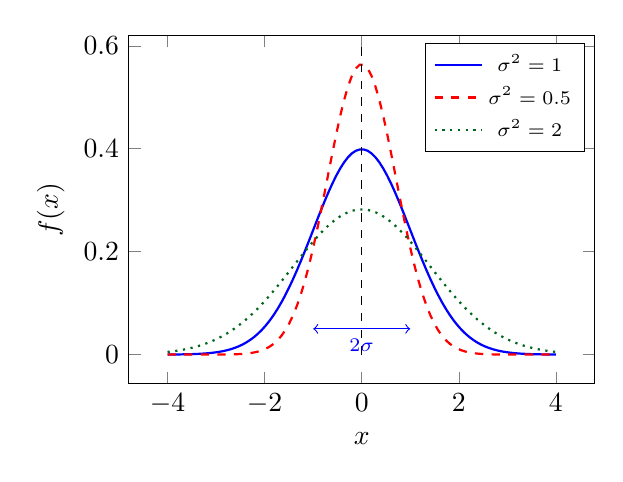
\begin{tikzpicture}
\begin{axis}[
  width=7.5cm, height=6cm,
  domain=-4:4, samples=100,
  xlabel={$x$}, ylabel={$f(x)$},
  legend style={at={(0.98,0.98)}, anchor=north east, font=\scriptsize},
  every axis plot/.append style={thick}
]
\addplot[blue] {exp(-x^2/2)/sqrt(2*pi)};
\addlegendentry{$\sigma^2=1$}
\addplot[red, dashed] {exp(-x^2/(2*0.5))/sqrt(2*pi*0.5)};
\addlegendentry{$\sigma^2=0.5$}
\addplot[darkgreen, dotted] {exp(-x^2/(2*2))/sqrt(2*pi*2)};
\addlegendentry{$\sigma^2=2$}
% Mark mean
\draw[black, thin, dashed] (axis cs:0,0) -- (axis cs:0,0.6);
\node[above] at (axis cs:0,0.6) {\scriptsize $\mu=0$};
% Mark sigma for standard normal
\draw[blue, <->] (axis cs:-1,0.05) -- (axis cs:1,0.05);
\node[blue, below] at (axis cs:0,0.05) {\scriptsize $2\sigma$};
\end{axis}
\end{tikzpicture}
\end{center}
\end{column}
\end{columns}
\end{frame}


\begin{frame}{Moment Conditions}

A parameter can be defined by an expectation it must satisfy.

\vspace{0.4cm}

\textbf{Example 1: Mean}

\[
\mathbb{E}[X - \mu] = 0.
\]

The true value of $\mu$ is the one that makes this expectation zero.

\vspace{0.4cm}

\textbf{Example 2: Linear Regression slope coefficients}

\[
\mathbb{E}\left[X (Y - X'\beta)\right] = 0.
\]

The true $\beta$ is the one that makes the regressors, X, uncorrelated
with the error $(Y-X'\beta).$

\vspace{0.4cm}

\end{frame}

\begin{frame}{General Form of Method of Moments}

Many models can be written as:

\[
\mathbb{E}[g(W, \theta)] = 0.
\]

\vspace{0.3cm}

\begin{itemize}
    \item $W$ = observable data.
    \item $\theta$ = parameter.
    \item $g(\cdot)$ encodes the economic or statistical restrictions.
\end{itemize}

\vspace{0.4cm}

Identification requires that these conditions determine a unique $\theta$.
\end{frame}
%%%%%%%%%%%%%%%%%%%%%%%%%%%%%%%%%%%%%%%%%%%%%%%%%%%%%
\section[CEF]{Joint, Marginal, and Conditional Distributions}
%%%%%%%%%%%%%%%%%%%%%%%%%%%%%%%%%%%%%%%%%%%%%%%%%%%%%

\begin{frame}
\frametitle{Joint Distributions}
Recall,
\begin{defn}
The joint distribution function of $(X,Y)$ is $F(x,y)=P[X\leq x,\ Y\leq y].$
\end{defn}
\begin{defn}
The joint density is
$f(x,y)=\frac{\partial^2}{\partial x \partial y} F(x,y).$
\end{defn}\pause
\bigskip
If our data is continuous, densities and distributions live in 3 (or higher) dimensions.
\end{frame}


\begin{frame}{Example: A Joint Density}
\begin{columns}
\column{0.5\textwidth}
Consider two parties (A, B) mobilizing voters, with $X+Y\leq 1$:
$$f(x,y)=6(1 - x - y),\quad x,y\geq 0$$
\begin{itemize}
\item Density is highest at $(0,0)$ and decreases as either party mobilizes more.
\item The 6 ensures $\int\int f(x,y)\,dx\,dy=1$:
$$\int_{0}^{1} \int_{0}^{1-x} 6(1 - x - y)\, dy\,dx=1$$
\end{itemize}
\column{0.5\textwidth}
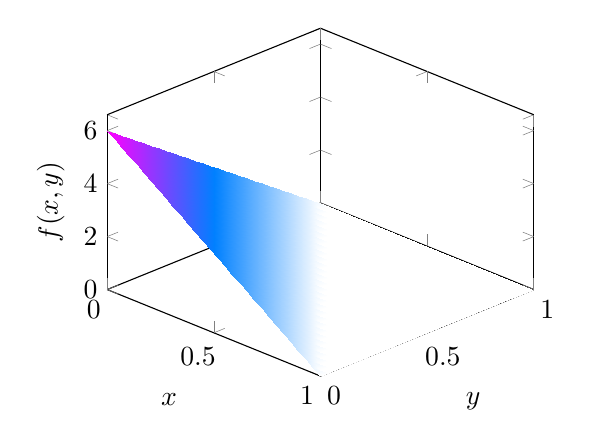
\begin{tikzpicture}
\begin{axis}[view={45}{35}, xlabel={$x$}, ylabel={$y$}, zlabel={$f(x,y)$}, domain=0:1, y domain=0:1, samples=30, samples y=30, zmin=0, colormap/cool, width=7cm, height=6cm]
\addplot3[surf, shader=interp]
{(x+y<=1)*(6*(1 - x - y))};
\end{axis}
\end{tikzpicture}
\end{columns}
\end{frame}


\begin{frame}{Marginal and Conditional Densities}
\begin{defn}
The \textbf{marginal density} of $X$ is
$$f_X(x)=\int_{-\infty}^\infty f(x,y)\,dy$$
\end{defn}
\begin{defn}
The \textbf{conditional density} of $Y$ given $X=x$ is
$$f_{Y|X}(y|x)=\frac{f(x,y)}{f_X(x)}$$
for any $x$ such that $f_X(x)>0$.
\end{defn}
These definitions are the bridge from joint distributions to regression.
\end{frame}


\begin{frame}{Example: Marginal and Conditional from $f(x,y)=6(1-x-y)$}
\textbf{Marginal density of $X$} fix x, integrate out $y$:
\begin{align*}
f_X(x)&=\int_0^{1-x}6(1-x-y)\,dy \pause
= 6\left[(1-x)y-\frac{y^2}{2}\right]_0^{1-x} \pause
= 3(1 - x)^2
\end{align*}\pause
\textbf{Conditional density of $Y|X=x$:}
\begin{align*}
f_{Y|X}(y|x)&=\frac{f(x,y)}{f_X(x)}=\frac{6(1-x-y)}{3(1-x)^2}=\frac{2(1-x-y)}{(1-x)^2}
\end{align*}\pause
Note: for each fixed $x$, this is a valid density in $y$ on $[0,\,1-x]$.
\end{frame}


%%%%%%%%%%%%%%%%%%%%%%%%%%%%%%%%%%%%%%%%%%%%%%%%%%%%%

%%%%%%%%%%%%%%%%%%%%%%%%%%%%%%%%%%%%%%%%%%%%%%%%%%%%%


\begin{frame}
\frametitle{Conditional Expectation}
$$\mathbb{E}[Y|X=x]=\int_{-\infty}^{\infty} y\, f_{Y|X}(y|x)\,dy=\frac{\int_{-\infty}^{\infty} y\, f(y,x)\,dy}{\int_{-\infty}^{\infty} f(y,x)\,dy}$$
\smallskip
\emph{The average value of $Y$ given that $X$ equals the specific value $x$.}
\end{frame}

\begin{frame}
\frametitle{Conditional Expectation Function (CEF)}
\begin{itemize}
\item \textbf{CEF}:
$$\mathbb{E}[Y|X=x]=m(x)$$
\item $Y$ is the dependent variable, $X=(X_1,\ldots, X_k)'$ are the independent variables.
\item $m(x)=\mathbb{E}[Y|X=x]$ is the value of a function at the real valued vector $x$.
\item $m(X)=\mathbb{E}[Y|X]$ is a function of random variables, so is itself a random variable.
\item We will show that the CEF is the best predictor of $Y$ given $X$ in the mean-square error sense.
\item In most applications we use a \emph{linear approximation} to the CEF, then make inferences about the joint distribution.
\end{itemize}
\end{frame}


\begin{frame}{Example: Computing the CEF from $f(x,y)=6(1-x-y)$}
\small
Apply the definition using our conditional density:
\begin{align*}
\mathbb{E}[Y|X=x]&=\int_0^{1-x} y\, f_{Y|X}(y|x)\,dy\\\pause
&=\int_0^{1-x} y\cdot\frac{2(1-x-y)}{(1-x)^2}\,dy\\\pause
&=\frac{2}{(1-x)^2}\int_0^{1-x} \left[(1-x)y-y^2\right]dy\\\pause
&=\frac{2}{(1-x)^2}\left[\frac{(1-x)y^2}{2}-\frac{y^3}{3}\right]_0^{1-x}\\\pause
&=\frac{2}{(1-x)^2}\left[\frac{(1-x)^3}{2}-\frac{(1-x)^3}{3}\right]
=\frac{2}{(1-x)^2}\cdot\frac{(1-x)^3}{6}\\\pause
&=\frac{1-x}{3}
\end{align*}
\end{frame}


\begin{frame}{Law of Iterated Expectations}
\begin{thm}
$\mathbb{E}[\mathbb{E}[Y|X]]=\mathbb{E}[Y]$,
\end{thm}
\small
\begin{align*}
\mathbb{E}[\mathbb{E}[Y|X]]&=\int_{-\infty}^\infty \mathbb{E}[Y|X=x]\,f_X(x)\,dx\\ \pause
&=\int_{-\infty}^\infty \int_{-\infty}^\infty y\,f_{Y|X}(y|x)\,dy\,f_X(x)\,dx\\\pause
&=\int_{-\infty}^\infty \int_{-\infty}^\infty y\,\frac{f(y,x)}{f_X(x)} f_X(x)\,dy\,dx\\\pause
&=\int_{-\infty}^\infty \int_{-\infty}^\infty y\,f(y,x)\,dy\,dx\\\pause
&=\int_{-\infty}^\infty y\, f_Y(y)\,dy=\mathbb{E}[Y]
\end{align*}
\end{frame}


\begin{frame}{Law of Total Variance}
\begin{thm}
$\text{Var}[Y]=\mathbb{E}[\text{Var}[Y|X]]+\text{Var}[\mathbb{E}[Y|X]]$
\end{thm}\pause
\begin{itemize}
\item $\text{Var}[\mathbb{E}[Y|X]]$: variance of the CEF --- the ``explained'' variance.
\item $\mathbb{E}[\text{Var}[Y|X]]$: average residual variance --- the ``unexplained'' variance.\pause
\item This decomposition underpins $R^2$: the fraction of the total variance of $Y$ explained by $X$.
\item You should be able to prove and apply both the LIE and LTV.
\end{itemize}
\end{frame}


\begin{frame}{Example: CEF from a Joint Density}
\begin{columns}
\column{0.45\textwidth}
Joint density:
$$f(x,y)=6(1 - x - y)$$
for $x\geq 0,\;y\geq 0,\;x+y\leq 1.$\\
\bigskip
Marginal:
$f_X(x)=3(1 - x)^2$\\
\bigskip
CEF:
$$\mathbb{E}(Y|X=x)=\frac{1-x}{3}$$
\column{0.55\textwidth}
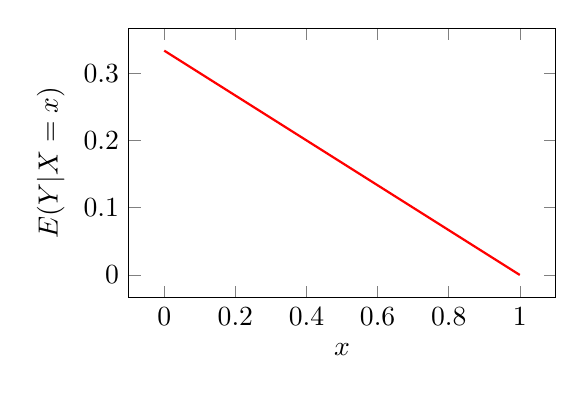
\begin{tikzpicture}
\begin{axis}[xlabel={$x$},ylabel={$\mathbb{E}(Y|X=x)$},domain=0:1,samples=100, width=7cm, height=5cm]
\addplot[color=red,thick]{(1 - x)/3};
\end{axis}
\end{tikzpicture}\\
\smallskip
As $X$ increases, $\mathbb{E}[Y|X]$ decreases linearly---this CEF \emph{is} linear.
\end{columns}
\end{frame}



%%%%%%%%%%%%%%%%%%%%%%%%%%%%%%%%%%%%%%%%%%%%%%%%%%%%%
\section[Matrices]{Matrix Algebra for Regression}
%%%%%%%%%%%%%%%%%%%%%%%%%%%%%%%%%%%%%%%%%%%%%%%%%%%%%


\begin{frame}{Linear Systems and Matrix Representation}
A system of linear equations
\begin{align*}
y_1&=\beta_0+\beta_1 x_{11}+\beta_2 x_{12}+\cdots\\
y_2&=\beta_0+\beta_1 x_{21}+\beta_2 x_{22}+\cdots\\
&\vdots
\end{align*}
can be written compactly as
$$\bm{y}=\bm{X}\bm{\beta}$$
where $\bm{y}$ is $n\times 1$, $\bm{X}$ is $n\times k$, and $\bm{\beta}$ is $k\times 1$.
\end{frame}

\begin{frame}{Matrix Multiplication}
If $\bm{A}$ is $k\times r$ and $\bm{B}$ is $r \times s$, they are \textbf{conformable} and
$$(\bm{AB})_{ij}=\sum_{\ell=1}^r a_{i\ell}\, b_{\ell j}$$
The result is $k \times s$.\\
\bigskip
Key rules:
\begin{itemize}
\item Generally $\bm{AB}\neq \bm{BA}$.
\item $\bm{A}(\bm{B}+\bm{C})=\bm{AB}+\bm{AC}$ \quad (distributive).
\item $(\bm{AB})\bm{C}=\bm{A}(\bm{BC})$ \quad (associative).
\item $(\bm{AB})'=\bm{B}'\bm{A}'$, where $'$ is the transpose.
\end{itemize}
\end{frame}


\begin{frame}{Inner Product and Similarity}
\begin{itemize}
\item The inner product of two $k\times 1$ vectors:
$$\bm{a}\cdot\bm{b}=\bm{a}'\bm{b}=\sum_{j=1}^k a_jb_j$$
\item Compare to covariance for demeaned variables:
$$\text{Cov}(\bm{x},\ \bm{y})=\frac{1}{n-1}\sum_{i=1}^n x_iy_i$$
\item Two vectors are \textbf{orthogonal} if $\bm{a}'\bm{b}=0$.
\item $||\bm{a}||=\sqrt{\bm{a}'\bm{a}}$ is the Euclidean norm (length) of $\bm{a}$.
\end{itemize}
\end{frame}


\begin{frame}{The Design Matrix $\bm{X}$}
In regression, $\bm{X}$ is the $n\times k$ \textbf{design matrix}: rows are observations, columns are variables.
$$\bm{X}=\begin{bmatrix}
1 & x_{11} & x_{12} & \cdots & x_{1,k-1}\\
1 & x_{21} & x_{22} & \cdots & x_{2,k-1}\\
\vdots & \vdots & \vdots & \ddots & \vdots\\
1 & x_{n1} & x_{n2} & \cdots & x_{n,k-1}
\end{bmatrix}
=\begin{bmatrix} \bm{x}_1' \\ \bm{x}_2' \\ \vdots \\ \bm{x}_n'\end{bmatrix}
=\begin{bmatrix} \bm{i} & \bm{c}_1 & \bm{c}_2 & \cdots & \bm{c}_{k-1}\end{bmatrix}$$\pause
\begin{itemize}
\item The first column $\bm{i}=(1,1,\ldots,1)'$ is the intercept.
\item Each row $\bm{x}_i'$ is observation $i$'s vector of regressors.
\item Each column $\bm{c}_j$ is the $n\times 1$ vector of all observations on variable $j$.
\item $\bm{X}$ has $n$ rows (observations) and $k$ columns (independent variables+intercept).
\end{itemize}
\end{frame}




\begin{frame}{Matrix Inverse}
\begin{itemize}
\item If a $k \times k$ matrix $\bm{A}$ is \emph{nonsingular} (full rank), there exists a unique $\bm{A}^{-1}$ such that $\bm{A}\bm{A}^{-1}=\bm{A}^{-1}\bm{A}=\bm{I}_k$.\pause
\item Key formulas:
\begin{itemize}
\item $(\bm{A}^{-1})'=(\bm{A}')^{-1}$
\item $(\bm{AB})^{-1}=\bm{B}^{-1}\bm{A}^{-1}$
\end{itemize}\pause
\item The \emph{rank} of a matrix is the number of linearly independent columns.
\item A matrix is singular (non-invertible) when its columns are linearly dependent---this corresponds to \textbf{perfect multicollinearity} in regression.
\end{itemize}
\end{frame}



%%%%%%%%%%%%%%%%%%%%%%%%%%%%%%%%%%%%%%%%%%%%%%%%%%%%%
\section[Pos. Definite]{Positive Definiteness and Quadratic Forms}
%%%%%%%%%%%%%%%%%%%%%%%%%%%%%%%%%%%%%%%%%%%%%%%%%%%%%


\begin{frame}{Quadratic Forms: An Example}
\begin{itemize}
\item We often want to characterize a 2nd degree polynomial like
\[
3x_1^2 + 4x_2^2 + 9x_3^2 - 5x_1x_3.
\]

\item We can write it as a quadratic form:
\[
\bm{x}^\top \bm{A} \bm{x}.
\]

\item The diagonal elements of $\bm{A}$ are the coefficients on $x_i^2$.

\item Cross terms are split across symmetric entries:
\[
-5x_1x_3 \Rightarrow a_{13}=a_{31}=-\frac{5}{2}.
\]

\item Thus,
\[
\bm{A}=
\begin{bmatrix}
3 & 0 & -\frac{5}{2} \\
0 & 4 & 0 \\
-\frac{5}{2} & 0 & 9
\end{bmatrix},
\qquad
\bm{x}=
\begin{bmatrix}
x_1\\
x_2\\
x_3
\end{bmatrix}.
\]

\end{itemize}
\end{frame}

\begin{frame}{Positive Definiteness}
\begin{itemize}
\item A \textbf{quadratic form} is a scalar $\bm{x}'\bm{A}\bm{x}$, where $\bm{A}$ is a symmetric matrix:
$$\bm{x}'\bm{A}\bm{x}=\sum_i a_{ii}x_i^2+2\sum_{i<j} a_{ij}x_ix_j$$\pause
\item A symmetric matrix $\bm{A}$ is \textbf{positive definite} if $\bm{c}'\bm{A}\bm{c}>0$ for all $\bm{c}\neq \bm{0}$.
\item A symmetric matrix $\bm{A}$ is \textbf{positive semi-definite} if $\bm{c}'\bm{A}\bm{c}\geq 0$ for all $\bm{c}\neq \bm{0}$.
\end{itemize}
\end{frame}

\begin{frame}{Why Positive Definiteness Matters}
\begin{columns}
\begin{column}{.55\textwidth}
\begin{itemize}
\item Variance-covariance matrices are positive semi-definite by construction.
\item If $\bm{X}$ has full column rank, $\bm{X}'\bm{X}$ is positive definite, guaranteeing a unique OLS solution.
\item PD allows us to compare matrices (which estimator has ``smaller'' variance):
$$\bm{A}-\bm{B} \text{ is PD} \implies \bm{A} \text{ is ``larger'' than } \bm{B}$$
\item A PD quadratic form is strictly convex with a unique global minimum---the OLS ``bowl.''
\end{itemize}
\end{column}
\begin{column}{.45\textwidth}
\begin{center}
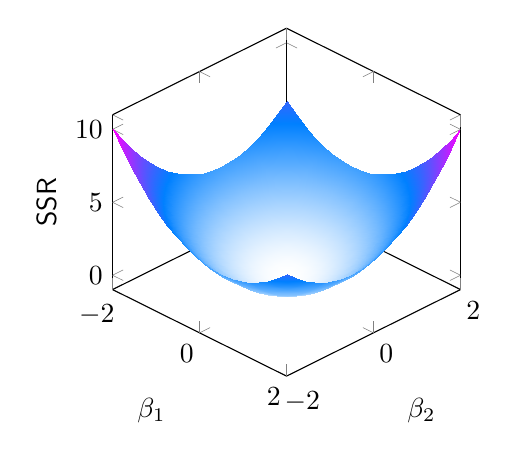
\begin{tikzpicture}
\begin{axis}[view={45}{35}, xlabel={$\beta_1$}, ylabel={$\beta_2$}, zlabel={SSR}, domain=-2:2, y domain=-2:2, samples=20, colormap/cool, width=6cm, height=6cm]
\addplot3[surf, shader=interp]{x^2 + y^2 + 0.5*x*y};
\end{axis}
\end{tikzpicture}
\end{center}
\end{column}
\end{columns}
\end{frame}


\begin{frame}{Reference: Properties of Positive Definite Matrices}
\begin{itemize}
\item $\bm{A}$ is PD $\iff$ it is symmetric with all eigenvalues positive.
\item If $\bm{A}$ is PD, it is nonsingular and $\bm{A}^{-1}$ is also PD.
\item If $\bm{A}$ is PD, $\text{tr}(\bm{A})>0$.
\item If $\bm{A}$ and $\bm{B}$ are PD, so is $\bm{A}+\bm{B}$.
\item If $\bm{A}$ is PD and $c>0$, then $c\bm{A}$ is PD.
\item If $\bm{A}$ is $n\times k$ with full column rank, then $\bm{A}'\bm{A}$ is PD.
\end{itemize}
\end{frame}

\begin{frame}{The Gram Matrix $\bm{X}'\bm{X}$}
\begin{align*}
\bm{X}'\bm{X}  = \begin{bmatrix} \sum x_{1i}^2 & \sum x_{1i}x_{2i}& \cdots\\
\sum x_{1i}x_{2i}& \sum x_{2i}^2  & \cdots\\
\vdots & \vdots & \ddots
  \end{bmatrix}
  \end{align*}
\begin{itemize}
  \item $\bm{X}'\bm{X}$ is symmetric and positive semi-definite.
  \item If we normalize columns so $||\bm{x}_j||=1$, then $(\bm{X}'\bm{X})_{ij}=\cos\theta_{ij}$: a measure of similarity.
  \item $\bm{X}'\bm{X}$ encodes all the second-moment information about the regressors.
\end{itemize}
\end{frame}

%%%%%%%%%%%%%%%%%%%%%%%%%%%%%%%%%%%%%%%%%%%%%%%%%%%%%
\section[Projection]{Vector Spaces and Projection}
%%%%%%%%%%%%%%%%%%%%%%%%%%%%%%%%%%%%%%%%%%%%%%%%%%%%%
\begin{frame}{Linear Combinations}

Given vectors $\bm{x}_1, \ldots, \bm{x}_k$,

a \textbf{linear combination} is any vector of the form

\[
c_1 \bm{x}_1 + \cdots + c_k \bm{x}_k.
\]

\vspace{0.4cm}

\textbf{Example in $\mathbb{R}^2$:}

\begin{itemize}
    \item One vector: all multiples lie on a line.
    \item Two non-collinear vectors: combinations fill the plane.
\end{itemize}

\vspace{0.4cm}

Linear combinations describe what vectors you can “build.”

\end{frame}

\begin{frame}{Span}

The \textbf{span} of $\bm{x}_1, \ldots, \bm{x}_k$ is

\[
\text{span}\{\bm{x}_1, \ldots, \bm{x}_k\}
=
\left\{
c_1 \bm{x}_1 + \cdots + c_k \bm{x}_k
\right\}.
\]

\vspace{0.4cm}

It is the set of *all* vectors you can build from them.

\vspace{0.4cm}

\textbf{Geometric intuition:}

\begin{itemize}
    \item One independent vector $\Rightarrow$ a line.
    \item Two independent vectors $\Rightarrow$ a plane.
    \item Three independent vectors in $\mathbb{R}^3$ $\Rightarrow$ all of $\mathbb{R}^3$.
\end{itemize}

\end{frame}
\begin{frame}{Linear Independence and Basis}

Vectors $\bm{x}_1, \ldots, \bm{x}_k$ are
\textbf{linearly independent} if

\[
c_1 \bm{x}_1 + \cdots + c_k \bm{x}_k = \bm{0}
\]

implies

\[
c_1 = \cdots = c_k = 0.
\]

\vspace{0.4cm}

Intuition:
\begin{itemize}
    \item No vector can be written as a combination of the others.
    \item No redundancy.
\end{itemize}

\vspace{0.4cm}

If independent vectors span a space $\mathcal{V}$,
they form a \textbf{basis}.

\end{frame}

\begin{frame}{Dimension and the Column Space}

\textbf{Dimension}

The dimension of a space is the number of vectors in any basis.

\vspace{0.4cm}

\textbf{In Regression}

\begin{itemize}
    \item The columns of $\bm{X}$ are your regressors.
    \item Their span is the \textbf{column space}.
    \item OLS projects $\bm{y}$ onto this space.
    \item Linear dependence $\Rightarrow$ no unique solution.
\end{itemize}

\vspace{0.4cm}

Full column rank = regressors are linearly independent.

\end{frame}


\begin{frame}{Projection: The Geometric Heart of OLS}
\begin{itemize}
    \item \textbf{Projection Theorem:} Let $\mathcal{W}$ be a subspace. There exists a unique $\hat{\bm{y}}\in \mathcal{W}$ closest to $\bm{y}$:
    $$\hat{\bm{y}} = \text{proj}_{\mathcal{W}}(\bm{y})$$\pause
    \item \textbf{Projection onto a line:} If $\mathcal{W}=\{c\,\bm{x}:c\in \mathbb{R}\}$, then
    $$\hat{\bm{y}} = \frac{\bm{x}'\bm{y}}{\bm{x}'\bm{x}}\,\bm{x}$$\pause
    \item \textbf{General case:} If $\mathcal{W}$ is the column space of $\bm{X}$, then
    $$\hat{\bm{y}} = \bm{X}(\bm{X}'\bm{X})^{-1}\bm{X}'\bm{y}\equiv \bm{P}\bm{y}$$
    where $\bm{P}=\bm{X}(\bm{X}'\bm{X})^{-1}\bm{X}'$ is the \textbf{hat matrix}.
    \end{itemize}
\end{frame}

\begin{frame}{Orthogonality of Residuals}
The error $\bm{e}=\bm{y}-\hat{\bm{y}}$ is orthogonal to every column of $\bm{X}$:
    \begin{align*}
      \bm{X}'(\bm{y}-\hat{\bm{y}}) &= \bm{X}'(\bm{y}-\bm{P}\bm{y})\\
      &= \bm{X}'\bm{y} - \bm{X}'\bm{X}(\bm{X}'\bm{X})^{-1}\bm{X}'\bm{y} \\
      &= \bm{X}'\bm{y} - \bm{X}'\bm{y} \\
      &= \bm{0}
    \end{align*}
\begin{itemize}
\item This is the matrix form of the OLS first-order conditions.
\item Geometrically: the residual vector is perpendicular to the column space of $\bm{X}$.
\item This is why $\sum_i \hat{e}_i = 0$ when there is an intercept (residuals are orthogonal to the column of ones).
\end{itemize}
\end{frame}




%%%%%%%%%%%%%%%%%%%%%%%%%%%%%%%%%%%%%%%%%%%%%%%%%%%%%
\section[Eigen/DoF]{Eigenvalues, Idempotent Matrices, and Degrees of Freedom}
%%%%%%%%%%%%%%%%%%%%%%%%%%%%%%%%%%%%%%%%%%%%%%%%%%%%%

\begin{frame}{Summarizing Matrices}

There are several useful summaries of a matrix $\bm{A}$:

\begin{itemize}
    \item \textbf{Trace:}
    \[
    \tr(\bm{A})=\sum_{i=1}^n A_{ii}
    \]
    \item \textbf{Determinant:} $\det(\bm{A})$ measures (signed) volume scaling; $\det(\bm{A})=0$ iff $\bm{A}$ is singular.
    \item \textbf{Rank:} $\rank(\bm{A})$ is the dimension of the column space.
    \item \textbf{Eigenvalues:} $\lambda_1,\ldots,\lambda_n$ summarize stretching along special directions.
\end{itemize}

\vspace{0.2cm}
We will use these repeatedly to diagnose invertibility and curvature.

\end{frame}


\begin{frame}{Properties of the Trace}
The trace has several properties that we will use repeatedly:
\begin{enumerate}
\item $\tr(\bm{A}+\bm{B})=\tr(\bm{A})+\tr(\bm{B})$ \hfill (linearity)
\item $\tr(c\bm{A})=c\,\tr(\bm{A})$ \hfill (linearity)
\item $\tr(\bm{A}'\!)=\tr(\bm{A})$ \hfill (transpose invariance)
\item $\tr(\bm{A}\bm{B})=\tr(\bm{B}\bm{A})$ \hfill (cyclic property)
\end{enumerate}
\bigskip
\textbf{Proof of (4):}
$\displaystyle\tr(\bm{A}\bm{B})=\sum_i(\bm{A}\bm{B})_{ii}=\sum_i\sum_j a_{ij}b_{ji}=\sum_j\sum_i b_{ji}a_{ij}=\sum_j(\bm{B}\bm{A})_{jj}=\tr(\bm{B}\bm{A})$
\bigskip

\textbf{Where this matters:} When we prove that $s^2=\frac{\bm{e}'\bm{e}}{n-k}$ is unbiased for $\sigma^2$, the key step uses
$$\mathbb{E}[\bm{e}'\bm{e}|\bm{X}]=\mathbb{E}[\tr(\bm{M}\bm{e}\bm{e}')|\bm{X}]=\tr(\bm{M}\,\mathbb{E}[\bm{e}\bm{e}'|\bm{X}])=\sigma^2\tr(\bm{M})=\sigma^2(n-k)$$
\end{frame}


\begin{frame}{Eigenvalues and Eigenvectors}

\begin{itemize}
\item For a square matrix $\bm{A}$, if
\[
\bm{A}\bm{u}=\lambda\bm{u}
\]
for some nonzero $\bm{u}$, then $\bm{u}$ is an \textbf{eigenvector} and $\lambda$ is the corresponding \textbf{eigenvalue}.\pause

\item Interpretation: along direction $\bm{u}$, the matrix acts like multiplication by $\lambda$.\pause

\item If $\bm{A}$ is symmetric, its eigenvalues are real and it has an orthonormal eigenbasis.\pause

\item Two useful identities:
\[
\tr(\bm{A})=\sum_{i=1}^n \lambda_i
\qquad\text{and}\qquad
\det(\bm{A})=\prod_{i=1}^n \lambda_i.\pause
\]

\item Eigenvalues diagnose key properties (symmetric $\bm{A}$):
\begin{itemize}
    \item $\lambda_i>0$ for all $i$ $\iff$ $\bm{A}$ is positive definite.
    \item Some $\lambda_i=0$ $\iff$ $\bm{A}$ is singular.
\end{itemize}

\end{itemize}

\end{frame}

\begin{frame}{Idempotent Matrices}

\begin{itemize}
\item A matrix is \textbf{idempotent} if
\[
\bm{A}^2=\bm{A}.
\]

\begin{thm}
If $\bm{A}$ is idempotent, then all eigenvalues of $\bm{A}$ are $0$ or $1$.
\end{thm}\pause

\item \textbf{Proof (one line):} If $\bm{A}\bm{x}=\lambda \bm{x}$, then
\[
\bm{A}^2\bm{x}=\lambda^2\bm{x}
\quad\text{but also}\quad
\bm{A}^2\bm{x}=\bm{A}\bm{x}=\lambda\bm{x},
\]
so $\lambda^2=\lambda$, hence $\lambda\in\{0,1\}$.\pause

\item The hat matrix
\[
\bm{P}=\bm{X}(\bm{X}'\bm{X})^{-1}\bm{X}'
\]
is symmetric and idempotent.\pause

\item $\rank(\bm{P})$ equals the number of eigenvalues equal to $1$ (so $\rank(\bm{P})=k$).\pause
\item Therefore $\tr(\bm{P})=k$.
\end{itemize}

\end{frame}

\begin{frame}{Orthogonal Complements and Dimension}

\begin{defn}
The \textbf{orthogonal complement} of a subspace $\mathcal{W}\subset \mathbb{R}^n$ is
\[
\mathcal{W}^{\perp}
=\{\bm{x}\in \mathbb{R}^n:\bm{x}'\bm{w}=0 \text{ for all }\bm{w}\in \mathcal{W}\}.
\]
\end{defn}\pause

\begin{thm}[Fundamental Theorem of Linear Algebra (dimension version)]
If $\mathcal{W}$ is a subspace of $\mathbb{R}^n$, then
\[
\dim(\mathcal{W})+\dim(\mathcal{W}^{\perp})=n.
\]
\end{thm}\pause

\textbf{Proof setup:} Let $\dim(\mathcal{W})=k$.
Choose an orthonormal basis $\bm{u}_1,\ldots,\bm{u}_k$ for $\mathcal{W}$.
Extend it to an orthonormal basis $\bm{u}_1,\ldots,\bm{u}_n$ for $\mathbb{R}^n$.

\end{frame}


\begin{frame}{Proof: $\dim(\mathcal{W})+\dim(\mathcal{W}^{\perp})=n$}

\textbf{Claim:} $\bm{u}_{k+1},\ldots,\bm{u}_n$ form a basis for $\mathcal{W}^{\perp}$, so $\dim(\mathcal{W}^{\perp})=n-k$.\pause

\vspace{0.2cm}

\textbf{Step 1 (orthogonality):}
For $j>k$ and $i\le k$, orthonormality gives $\bm{u}_j'\bm{u}_i=0$, hence $\bm{u}_j\in\mathcal{W}^{\perp}$.\pause

\vspace{0.2cm}

\textbf{Step 2 (spanning):}
Take any $\bm{v}\in\mathcal{W}^{\perp}$ and expand in the full basis:
\[
\bm{v}=\sum_{i=1}^n c_i\bm{u}_i.
\]\pause
For any $j\le k$,
\[
0=\bm{v}'\bm{u}_j=c_j,
\]
so $\bm{v}=\sum_{i=k+1}^n c_i\bm{u}_i$, which lies in $\spn\{\bm{u}_{k+1},\ldots,\bm{u}_n\}$.\pause

\vspace{0.2cm}

\textbf{Step 3 (independence):}
$\bm{u}_{k+1},\ldots,\bm{u}_n$ are orthonormal, hence linearly independent.\pause

\vspace{0.2cm}

Therefore $\dim(\mathcal{W}^{\perp})=n-k$, so $\dim(\mathcal{W})+\dim(\mathcal{W}^{\perp})=k+(n-k)=n.\ \square$

\end{frame}


\begin{frame}{Degrees of Freedom}

Let $\mathcal{W}=\col(\bm{X})$ be the column space of $\bm{X}$.

\begin{itemize}
    \item $\dim(\mathcal{W})=k$ (number of linearly independent regressors).\pause
    \item The fitted values satisfy $\hat{\bm{y}}\in\mathcal{W}$.\pause
    \item The residuals satisfy $\hat{\bm{u}}=\bm{y}-\hat{\bm{y}}\in \mathcal{W}^{\perp}$.\pause
    \item By $\dim(\mathcal{W})+\dim(\mathcal{W}^{\perp})=n$,
    \[
    \dim(\mathcal{W}^{\perp})=n-k.
    \]\pause
    \item This is why we divide by $n-k$ when estimating $\sigma^2$:
    residual variation lives in an $(n-k)$-dimensional space.
\end{itemize}

\end{frame}
%%%%%%%%%%%%%%%%%%%%%%%%%%%%%%%%%%%%%%%%%%%%%%%%%%%%%
\section[Vector Calculus]{Calculus with Vectors and Matrices}
%%%%%%%%%%%%%%%%%%%%%%%%%%%%%%%%%%%%%%%%%%%%%%%%%%%%%

\begin{frame}{What Is the Derivative of a Vector Function?}

Let $f(a_1, a_2, a_3, \ldots a_k)=f(\bm{a})$ be a scalar function of a vector
$\bm{a} \in \mathbb{R}^k$.

\vspace{0.3cm}

The \textbf{gradient} is:

\[
\nabla_{\bm{a}} f(\bm{a})
=
\begin{bmatrix}
\dfrac{\partial f}{\partial a_1} \\
\vdots \\
\dfrac{\partial f}{\partial a_k}
\end{bmatrix}.
\]

\vspace{0.4cm}

\textbf{Key idea:}

\begin{itemize}
    \item Derivative of a scalar w.r.t. a vector is a vector.
    \item First-order condition for a minimum:
    \[
    \nabla_{\bm{a}} f(\bm{a}) = \bm{0}.
    \]
\end{itemize}

\end{frame}

\begin{frame}{Linear Forms}

Let $f(\bm{a}) = \bm{z}'\bm{a}$,
where $\bm{z}$ is fixed.

\vspace{0.3cm}

Write it out:
\[
f(\bm{a}) = \sum_{j=1}^k z_j a_j.
\]

\vspace{0.3cm}

Taking derivatives componentwise:

\[
\nabla_{\bm{a}} (\bm{z}'\bm{a}) = \bm{z}.
\]

\vspace{0.5cm}

More generally, if $f(\bm{a}) = \bm{Z}\bm{a}$,

\[
\dfrac{d\,\bm{Z}\bm{a}}{d\,\bm{a}} = \bm{Z}.
\]

\end{frame}

\begin{frame}{Derivatives of Quadratic Forms}

Let
\[
f(\bm{a}) = \bm{a}'\bm{Z}\bm{a}.
\]

\vspace{0.3cm}

Write it out:
\[
f(\bm{a}) = \sum_{i,j} a_i Z_{ij} a_j.
\]

\vspace{0.4cm}

Taking derivatives:

\[
\nabla_{\bm{a}} (\bm{a}'\bm{Z}\bm{a})
=
(\bm{Z} + \bm{Z}')\bm{a}.
\]

\vspace{0.3cm}

If $\bm{Z}$ is symmetric, so $\bm{Z}=\bm{Z}'$ :

\[
\nabla_{\bm{a}} (\bm{a}'\bm{Z}\bm{a})
=
2\bm{Z}\bm{a}.
\]

\end{frame}

\begin{frame}{Application: Deriving OLS}

Least squares solves:

\[
\min_{\bm{\beta}}
(\bm{y} - \bm{X}\bm{\beta})'
(\bm{y} - \bm{X}\bm{\beta}).
\]

\vspace{0.4cm}

Expand:

\[
=
\bm{y}'\bm{y}
- 2\bm{\beta}'\bm{X}'\bm{y}
+ \bm{\beta}'\bm{X}'\bm{X}\bm{\beta}.
\]

\vspace{0.4cm}

Take gradient and set equal to zero:

\[
-2\bm{X}'\bm{y}
+ 2\bm{X}'\bm{X}\bm{\beta}
= \bm{0}.
\]

\vspace{0.3cm}

\[
\Rightarrow
\hat{\bm{\beta}} =
(\bm{X}'\bm{X})^{-1}\bm{X}'\bm{y}.
\]

\end{frame}

\begin{frame}{Second-Order Condition: Verifying a Minimum}
The FOC gave us a critical point.  Is it a minimum?
\bigskip

The \textbf{Hessian} (matrix of second derivatives) of $(\bm{y}-\bm{X}\bm{\beta})'(\bm{y}-\bm{X}\bm{\beta})$ is:
$$\frac{\partial^2}{\partial \bm{\beta}\,\partial \bm{\beta}'}\left[\bm{y}'\bm{y}-2\bm{\beta}'\bm{X}'\bm{y}+\bm{\beta}'\bm{X}'\bm{X}\bm{\beta}\right]=2\bm{X}'\bm{X}$$

\begin{itemize}
\item If $\bm{X}$ has full column rank, then $\bm{X}'\bm{X}$ is positive definite (from our earlier result).
\item A positive definite Hessian means the objective is strictly convex --- the critical point is a unique global minimum.
\item This connects two sections: positive definiteness guarantees both that $(\bm{X}'\bm{X})^{-1}$ exists \emph{and} that the solution is a minimum.
\end{itemize}
\end{frame}

%%%%%%%%%%%%%%%%%%%%%%%%%%%%%%%%%%%%%%%%%%%%%%%%%%%%%
\section[Roadmap]{Looking Ahead}
%%%%%%%%%%%%%%%%%%%%%%%%%%%%%%%%%%%%%%%%%%%%%%%%%%%%%


\begin{frame}{Summary and Roadmap}
\begin{itemize}
\item The \textbf{CEF} $\mathbb{E}[Y|\bm{X}=\bm{x}]$ is the target of regression---the best MSE predictor.
\item \textbf{OLS} is the linear approximation: a projection of $\bm{y}$ onto the column space of $\bm{X}$.
\item The OLS residual is orthogonal to $\bm{X}$ (first-order conditions).
\item Positive definiteness of $\bm{X}'\bm{X}$ guarantees existence and uniqueness.
\item Degrees of freedom ($n-k$) come from the rank-nullity theorem.
\bigskip
\item \textbf{Next:} the CEF vs Best Linear Predictor
\end{itemize}
\end{frame}



\end{document}
